\documentclass[border=4pt]{standalone}
% Shared TikZ macros for the "Gaussian wave" amplitude diagrams.
% Each wave is drawn isolated inside a fixed-size cell, no axes, with an
% optional probability label placed just outside the bump.
\usepackage{tikz}
\usepackage{amssymb}
\usepackage{amsmath}
\usetikzlibrary{calc,arrows.meta}

\definecolor{waveblue}{HTML}{3A7CA5}
\definecolor{wavered}{HTML}{D1495B}

% \gaussiancell{x0}{y0}{sign}{height}{color}{basislabel}{highlight}{problabel}
% Draws one Gaussian bump centered at (x0,y0), cell width 2.4, height range +-1.1.
% sign: +1 upright, -1 flipped. height: 0..1 (fraction of max bump height 0.85).
% basislabel: basis-state ket, always placed BELOW the baseline; empty string = no label.
% highlight: 1 draws a thin colored box around the cell, 0 = none.
% problabel: probability value, always placed ABOVE the bump's peak; empty string = no label.
\newcommand{\gaussiancell}[8]{%
  \begin{scope}[shift={(#1,#2)}]
    \pgfmathsetmacro{\amp}{#4*0.85*#3}
    \pgfmathsetmacro{\wid}{0.30}
    \draw[black, line width=0.5pt] (-1.15,0) -- (1.15,0);
    \draw[#5, line width=1.3pt, samples=120, smooth, domain=-1.05:1.05]
      plot (\x, {\amp*exp(-(\x*\x)/(2*\wid*\wid))});
    \fill[#5, opacity=0.18, samples=120, domain=-1.05:1.05]
      plot (\x, {\amp*exp(-(\x*\x)/(2*\wid*\wid))}) -- (1.05,0) -- (-1.05,0) -- cycle;
    \ifnum#7=1
      \draw[wavered, line width=0.9pt] (-1.15,-0.65) rectangle (1.15,1.35);
    \fi
    \ifx&#6&
    \else
      \ifnum#3>0
        \node[anchor=north, font=\footnotesize] at (0, -0.35) {#6};
      \else
        \node[anchor=north, font=\footnotesize] at (0, -0.95) {#6};
      \fi
    \fi
    \ifx&#8&
    \else
      \node[anchor=south, font=\small] at (0, 0.95) {#8};
    \fi
  \end{scope}
}

% \wavegrid{rows}{cols}{dx}{dy}{cellfn} where cellfn takes (row,col,index)
% (grid layout handled inline per-figure instead, for full control over per-cell content)

% \meanline{x0}{y0}{width}{amp}{label}
% Draws a dotted horizontal line at height amp (in the same units as
% \gaussiancell's amplitude, i.e. peak height = 0.85 at amp=1) spanning
% `width` cells wide, centered at (x0,y0), with a small label to its right.
\newcommand{\meanline}[5]{%
  \begin{scope}[shift={(#1,#2)}]
    \pgfmathsetmacro{\amp}{#4*0.85}
    \draw[gray, line width=0.9pt, densely dotted] (-1.15,\amp) -- (#3-1.15,\amp);
    \ifx&#5&
    \else
      \node[gray, anchor=west, font=\footnotesize] at (#3-1.05,\amp) {#5};
    \fi
  \end{scope}
}

\begin{document}
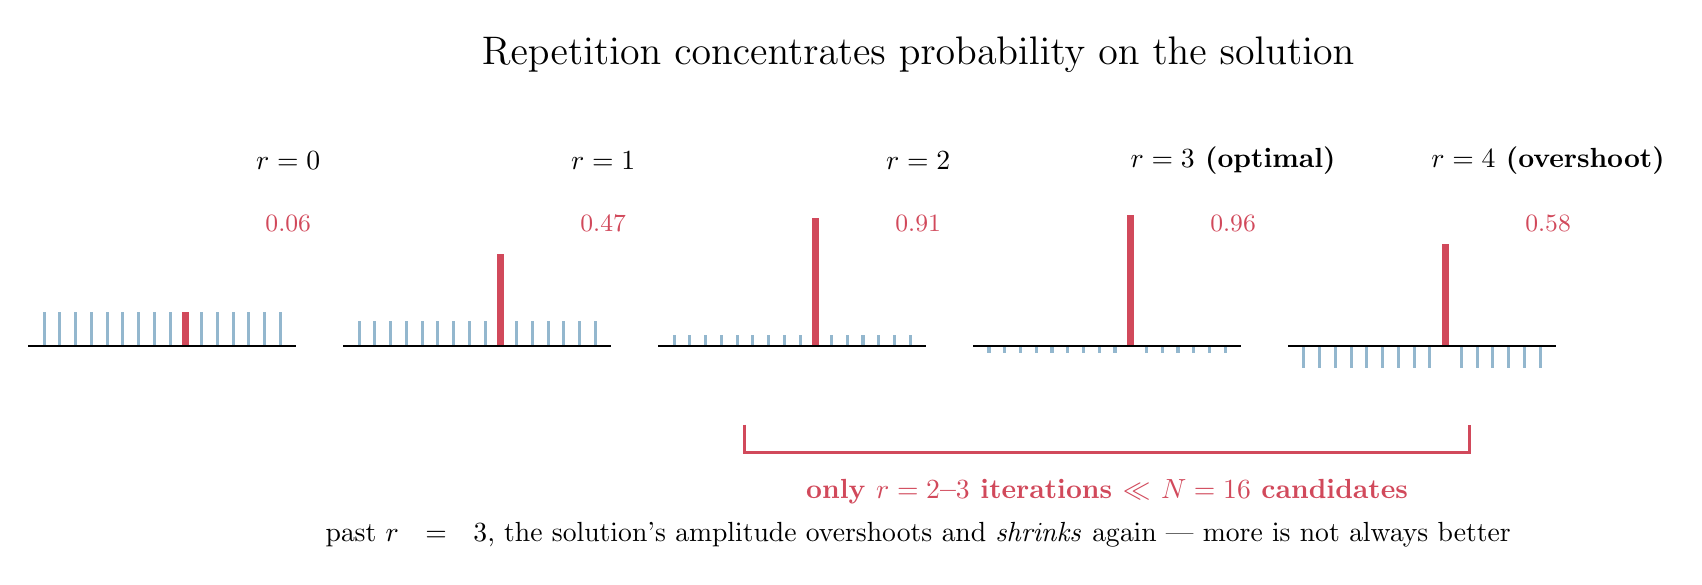
\begin{tikzpicture}
  \node[font=\Large] at (9.6, 3.7) {Repetition concentrates probability on the solution};

  % \iterpanel{x0}{r label}{amp_w}{prob_w}{amp_o}
  % One small panel: 16 tiny bars, winner highlighted, with the winner's
  % amplitude sign shown by bar direction and probability labeled above.
  \newcommand{\iterpanel}[5]{%
    \begin{scope}[shift={(#1,0)}]
      \node[font=\normalsize\bfseries] at (1.6,2.35) {#2};
      \foreach \i in {0,...,15} {
        \pgfmathsetmacro{\barx}{-1.5+\i*0.2}
        \ifnum\i=9
          \pgfmathsetmacro{\bary}{#3*1.7}
          \draw[wavered, line width=2.6pt] (\barx,0) -- (\barx,\bary);
        \else
          \pgfmathsetmacro{\bary}{#5*1.7}
          \draw[waveblue, line width=1.1pt, opacity=0.55] (\barx,0) -- (\barx,\bary);
        \fi
      }
      \draw[black, line width=0.5pt] (-1.7,0) -- (1.7,0);
      \node[wavered, font=\small] at (1.6,1.55) {$#4$};
    \end{scope}
  }

  \iterpanel{0}{$r=0$}{0.25}{0.06}{0.25}
  \iterpanel{4}{$r=1$}{0.6875}{0.47}{0.1875}
  \iterpanel{8}{$r=2$}{0.9531}{0.91}{0.0781}
  \iterpanel{12}{$r=3$ (optimal)}{0.9805}{0.96}{-0.0508}
  \iterpanel{16}{$r=4$ (overshoot)}{0.7627}{0.58}{-0.167}

  % ---------- Callout: r=2,3 reach high probability using far fewer than N=16 tries ----------
  \draw[wavered, line width=1.1pt] (7.4,-1.0) -- (7.4,-1.35) -- (16.6,-1.35) -- (16.6,-1.0);
  \node[wavered, font=\normalsize\bfseries] at (12.0,-1.85)
    {only $r=2$--$3$ iterations $\ll$ $N=16$ candidates};

  \node[font=\normalsize, text width=18.5cm, align=center] at (9.6, -2.4)
    {past $r=3$, the solution's amplitude overshoots and \emph{shrinks} again --- more is not always better};
\end{tikzpicture}
\end{document}
